\chapter{Investigated approach}

\section{Data}

The primary dataset utilized in this study is the LIDC-IDRI (Lung Image Database Consortium and Image Database Resource Initiative) dataset. As a premier public resource for lung nodule analysis, it provides a comprehensive collection of thoracic CT scans, unblinded radiologist annotations, and clinical diagnostic records. Because nodules are frequently reviewed by multiple radiologists, the dataset captures inherent clinical variability and uncertainty, making it highly representative of real-world diagnostic scenarios. For this analysis, the data is divided into three interconnected components: the raw imaging data, the clinical diagnosis records and the nodule annotations.

\subsection{Radiological Imaging Data}
The imaging data consists of 3D CT scans stored as raw DICOM files. The pipeline recursively extracts files with the ``CT'' modality and reconstructs the full axial chest volume by sorting the 2D slices along the Z-axis (utilizing spatial attributes such as ImagePositionPatient). Each 2D slice has a standard image size of 512x512 pixels. To ensure accurate radiodensity representations, the raw pixel arrays are converted into standardized Hounsfield Units (HU) using the RescaleSlope and RescaleIntercept metadata.

\subsection{Radiologist Nodule Annotations}
Accompanying the DICOM files are XML annotation files documenting findings from radiologist reading sessions. These annotations describe the location, size, shape, internal structure, margin sharpness, and visual appearance of the identified lesions. A critical characteristic extracted for this study is the nodule texture, which indicates how dense or solid a lesion appears on a CT scan.

The original texture scores in the dataset range from 1 to 5, each corresponding to the following labels, in order: non-solid, mostly non-solid, part-solid, mostly solid, solid

To reduce noise and facilitate comparative analysis, these scores were mapped into three distinct radiological categories:

Ground-Glass (Scores 1 \& 2): Lighter, less dense regions.

Part-Solid (Score 3): Lesions containing both dense and non-dense regions.

Solid (Scores 4 \& 5): Denser, brighter regions.

\subsection{Clinical Diagnosis Data}
A supplementary clinical dataset provides patient and nodule-level diagnostic context across 157 patient records. This component contains variables detailing clinical outcomes, including the overall diagnosis result, tumor location, and the specific method used to confirm the diagnosis (e.g., biopsy, surgical resection, radiological follow-up, or progression). For metastatic cases, the primary tumor site is recorded across 112 unique classes (e.g., non-small cell lung cancer, melanoma, colon cancer).

\subsection{Data Processing and Feature Engineering}
To structure the data for modeling, the annotation data was aggregated into two distinct relational tables.

One is a detailed table with one row for each texture annotation, containing the following information: Patient ID, Nodule ID, Reading session index, Texture score and Texture category.

The other table is a patient-level summary table that combines all annotations for a patient and stores the following data: Total number of texture annotations, Number of ground-glass nodules, Number of part-solid nodules, Number of solid nodules, Dominant texture category.

The dominant texture category is the one that appears most often for that patient. For example, if most nodules for a patient are solid, then the patient is labeled as having a dominant solid texture pattern.

\subsection{Machine Learning Target Variables}
Predicting exact medical diagnoses across highly granular classes is challenging, particularly given the sample size constraints of the clinical dataset. To create robust predictive models, the clinical labels were simplified into three distinct binary and multiclass targets, focusing on the most critical medical distinctions:

\textbf{Malignancy prediction}: 0 for benign (derived from ``benign/non-malignant'' labels) and 1 for malignant (derived from ``malignant primary lung cancer'' and ``malignant metastatic lesion'' labels);

\textbf{Progression prediction}: 0 for stable (nodule remained stable for at least two years) and 1 for progressive (documented progression);

\textbf{Radiological subtype}: as previously mentioned: 0 for solid, 1 for part-solid and 2 for ground-glass

This makes the classification problem easier and helps the model focus on the most important medical distinction: whether the nodule is dangerous or not.

\subsection{Exploratory Data Analysis}

After extracting and inspecting the data, several properties relevant to modeling were identified.

Regarding texture distribution, solid nodules are by far the most frequent category, followed by ground-glass and part-solid. This class imbalance is consistent with clinical literature and must be accounted for during training. Furthermore, most CT series contain only one or two annotated nodules. The distribution of nodule counts per scan is heavily right-skewed, meaning a small number of scans account for a disproportionately large share of the total annotations.

Because each patient may have been reviewed by up to four radiologists in separate reading sessions, the same nodule can receive different texture scores from different readers. This inter-reader variability was partially mitigated at the patient level by applying a majority-vote approach to establish a single ``dominant texture category'' across all annotations.

In the diagnosis dataset, the nodule-level columns for higher-indexed nodules (e.g., nodules 4 and 5) contain a massive fraction of missing values, reflecting the fact that most patients have fewer than four annotated nodules. Additionally, the \texttt{primary\_tumor\_site} column was excluded as a feature; it applies specifically to metastatic cases and suffers from extreme high cardinality (containing over 110 unique free-text classes for just 157 patients), rendering it too fragmented for robust model training.

Finally, both derived classification targets exhibit class imbalance. The malignancy target is moderately skewed toward the benign class, while the progression target is severely unbalanced, with stable cases substantially outnumbering progressive ones. 

Overall, the dataset is valuable because it combines CT images, radiologist annotations, and diagnosis information. This supports both exploratory analysis and predictive modeling. Furthermore, the presence of missing values, annotation variability, and multiple expert opinions makes the dataset more representative of real clinical scenarios.

\section{Proposed Architecture}
\label{section:proposedArchitecture}

To address the problem of simultaneous texture, malignancy, and progression classification, we propose a multi-task learning architecture termed \textit{MultiTaskCrossTalkNet}. The primary objective of this architecture is to evaluate the efficacy of simultaneously predicting a nodule's physical texture, its immediate malignancy risk, and its long-term clinical progression. Specifically, the network relies on the hypothesis that soft parameter sharing (cross-talk) between these three highly correlated clinical tasks improves overall diagnostic performance compared to isolating them. Because physical composition, cancer risk, and growth rate are biologically linked, allowing the model to share learned feature representations should theoretically yield a more robust predictive model.

Instead of hard parameter sharing (which forces all tasks to use the exact same early-layer weights), this proposed network employs three parallel Convolutional Neural Network (CNN) branches: one dedicated to texture, one to malignancy, and one to progression. After each convolutional block, a learnable \textit{CrossStitchUnit} linearly combines the activation maps across the parallel branches. This allows the network to dynamically learn how much information to share between the tasks at varying levels of abstraction.

The network is designed to output three predictions from its respective classification heads:

1. A 3-class target for the dominant texture category (ground-glass, part-solid, solid), represented via one-hot encoding.

2. A binary target representing the nodule's immediate risk level (0 for benign, 1 for malignant).

3. A binary target representing the nodule's longitudinal progression (0 for stable, 1 for progressive).

The three-task formulation above describes the full, intended design of \textit{MultiTaskCrossTalkNet}, with one branch per task and a learnable cross-stitch matrix whose size matches the number of active tasks. As explained in the Scope and Limitations discussion of Section~\ref{section:experimentsAndResults}, the progression task (T2) could not be reliably linked to the imaging data and therefore had to be excluded from every experiment. All results reported in this chapter are consequently for the resulting two-task instantiation: a texture branch and a malignancy branch, coupled by a $2 \times 2$ cross-stitch matrix after each convolutional block.


\section{Experiments and Results}
\label{section:experimentsAndResults}

\subsection{Single-Task Learning (STL)}

The STL baseline consists of two independently trained CNN models: one for texture classification and one for malignancy prediction, that share no parameters and receive no signal from one another. Each model is architecturally identical to a single branch of the full \textit{MultiTaskCrossTalkNet}, with the cross-stitch units removed and a single task-specific classification head attached directly to the final convolutional block. This design ensures that any performance difference between STL and MTL is attributable solely to the cross-talk mechanism, and not to differences in feature extraction capacity.

The same preprocessing pipeline, train/validation/test split, and AdamW optimiser were applied as in the MTL experiments, so results are directly comparable. Each model was trained to minimise its respective loss function independently: categorical cross-entropy for the texture model and binary cross-entropy for the malignancy model. The best-performing checkpoint was selected based on lowest validation loss and subsequently evaluated on the held-out test set.

\subsubsection{Preliminary Experiment (15 samples)}

An initial feasibility run was conducted on a severely restricted subset of 15 annotated samples to validate the training pipeline end-to-end before scaling up.

The malignancy STL model achieved a test accuracy of 66.67\%, with a macro-averaged F1 of 0.40 (loss: 1.2636). The model entirely failed to identify the benign class (precision, recall, and F1 all 0.00; support: 1), while achieving an F1 of 0.80 on the malignant class (precision: 0.67, recall: 1.00; support: 2). This pattern is consistent with a near-degenerate predictor biased toward the majority class.

The texture STL model achieved a test accuracy of 100\% and a loss of 0.0018, but a macro-averaged F1 of only 0.33. This apparent contradiction is fully explained by the composition of the test set: all three test samples belonged to the solid class (support: 3/0/0), so a majority-class predictor achieves perfect accuracy while producing zero precision and recall for ground-glass and part-solid. These results are therefore not meaningful and serve only to confirm pipeline correctness.

\subsubsection{Full Experiment (508 samples)}

The full experiment used 508 samples, partitioned into training (306), validation (101), and test (101) sets.

The malignancy STL model achieved a test accuracy of 61.39\% and a macro-averaged F1 of 0.56 (loss: 0.6808). Per-class results are reported in Table~\ref{tab:stl_malignancy_full}. The model demonstrated substantially better recall for the malignant class (0.82) than for the benign class (0.32), consistent with an imbalance-driven bias toward the more frequent positive class.

\begin{table}[h]
\centering
\caption{Per-class metrics for the STL malignancy model, full experiment
  (held-out test set, $n=101$).}
\label{tab:stl_malignancy_full}
\begin{tabular}{lcccc}
\hline
\textbf{Class} & \textbf{Precision} & \textbf{Recall} & \textbf{F1}
  & \textbf{Support} \\
\hline
Benign    & 0.5417 & 0.3171 & 0.4000 & 41 \\
Malignant & 0.6364 & 0.8167 & 0.7153 & 60 \\
\hline
\textbf{Macro avg} & 0.5890 & 0.5669 & 0.5577 & 101 \\
\hline
\end{tabular}
\end{table}

The texture STL model achieved a test accuracy of 96.04\% and a macro-averaged F1 of 0.33 (loss: 0.1671). As in the preliminary run, the macro F1 is severely deflated by the class imbalance in the test set: 97 of 101 samples belong to the solid class, leaving only 2 ground-glass and 2 part-solid samples. The model correctly classifies all solid nodules (F1: 0.9798) but predicts nothing for the minority classes. Per-class results are reported in Table~\ref{tab:stl_texture_full}.

\begin{table}[h]
\centering
\caption{Per-class metrics for the STL texture model, full experiment
  (held-out test set, $n=101$).}
\label{tab:stl_texture_full}
\begin{tabular}{lcccc}
\hline
\textbf{Class} & \textbf{Precision} & \textbf{Recall} & \textbf{F1}
  & \textbf{Support} \\
\hline
Ground-glass & 0.0000 & 0.0000 & 0.0000 & 2 \\
Part-solid   & 0.0000 & 0.0000 & 0.0000 & 2 \\
Solid        & 0.9604 & 1.0000 & 0.9798 & 97 \\
\hline
\textbf{Macro avg} & 0.3201 & 0.3333 & 0.3266 & 101 \\
\hline
\end{tabular}
\end{table}

These results establish a task-isolated performance baseline against which the multi-task architectures are evaluated in the following subsection.



\subsection{Multi-Task Learning (MTL) with Cross-Talk}

\subsubsection{Scope and Limitations}

The original design of \textit{MultiTaskCrossTalkNet} targeted three simultaneous tasks: texture classification, malignancy prediction, and longitudinal progression prediction. In practice, the three-task formulation could not be implemented as intended due to a data linkage constraint: the clinical diagnosis file, which contains progression labels, does not share a common patient or nodule identifier with the DICOM XML annotation files from which texture and imaging features are derived. Without a reliable key with which to join these two sources, progression labels could not be unambiguously matched to individual CT crops, making it impossible to include the progression head in any image-driven training pipeline.

Beyond this linkage issue, the progression target is severely class-imbalanced (stable cases substantially outnumbering progressive ones), and predicting longitudinal temporal change from a single static cross-sectional slice presents fundamental modelling challenges. Preliminary tests confirmed that noisy gradients from a progression branch actively degraded the convergence of the other two tasks. The final experiments were therefore limited to the two-task setting: dominant texture category and binary malignancy.

\subsubsection{Experimental Setup}

To prepare inputs for the two-branch networks, a preprocessing pipeline was applied to the raw DICOM files. For each nodule, a representative 2D frame was extracted by selecting the middle slice of the nodule's spatial sequence using the SOP UID\@. Pixel arrays were transformed using the DICOM \texttt{RescaleSlope} and \texttt{RescaleIntercept} attributes, clipped to a Hounsfield Unit (HU) range of $[-1000, 400]$, and normalised to a $[0, 1]$ scale. Images were then cropped around the region-of-interest (ROI) bounding box with a predefined margin and resized to $128 \times 128$ pixels.

The dataset was partitioned into training (60\%), validation (20\%), and test (20\%) sets. All MTL variants were trained using the AdamW optimiser to minimise a joint loss: the weighted sum of categorical cross-entropy for the texture head and binary cross-entropy for the malignancy head, with both task weights set to 1.0. The best-performing checkpoint was selected on lowest validation loss and evaluated on the held-out test set.

Two MTL variants were implemented and compared:

\begin{itemize}
  \item \textbf{Cross-stitch:} Each branch exchanges information with the other via a learnable $2 \times 2$ mixing matrix inserted after every convolutional block. The matrix linearly combines the full activation tensors of both streams, with weights initialised to favour task-private representations (0.9 on the diagonal, 0.1 off-diagonal) and refined during training.

  \item \textbf{Co-attention:} Each branch derives a channel-wise gate by globally average-pooling the \textit{other} branch's feature map into a descriptor vector, then passing it through a small squeeze-and-excitation MLP (reduction ratio 8) with a Sigmoid output. The resulting gate is broadcast back to full spatial resolution and used to scale the other branch's features before adding them as a residual to the current branch. This allows each stream to selectively attend to the channels of the other that are most relevant to its own task, rather than mixing all channels uniformly. As with the cross-stitch unit, co-attention units are inserted after each of the three convolutional blocks, prior to max-pooling.
\end{itemize}

\subsubsection{Preliminary Experiment (15 samples)}

As with the STL models, a preliminary run on 15 samples was conducted to validate the joint training pipeline. The MTL cross-stitch model achieved a combined test loss of 1.1490. Texture accuracy was 100\% (macro F1: 0.33) and malignancy accuracy was 66.67\% (macro F1: 0.40). The per-class breakdown mirrors the STL results exactly: the texture head collapses to a solid-only predictor due to the degenerate test set composition, and the malignancy head fails to identify benign cases. No meaningful comparison between STL and MTL can be drawn at this scale.

\subsubsection{Full Experiment Results (508 samples)}

Results for both MTL variants on the full dataset are reported in Tables~\ref{tab:mtl_texture_full} and~\ref{tab:mtl_malignancy_full}, alongside the STL baseline for direct comparison.

\begin{table}[h]
\centering
\caption{Texture head performance across all models, full experiment (held-out test set, $n=101$). STL results repeated from Table~\ref{tab:stl_texture_full} for comparison.}
\label{tab:mtl_texture_full}
\begin{tabular}{llcccc}
\hline
\textbf{Model} & \textbf{Class} & \textbf{Precision} & \textbf{Recall}
  & \textbf{F1} & \textbf{Support} \\
\hline
\multirow{4}{*}{STL}
  & Ground-glass & 0.0000 & 0.0000 & 0.0000 & 2 \\
  & Part-solid   & 0.0000 & 0.0000 & 0.0000 & 2 \\
  & Solid        & 0.9604 & 1.0000 & 0.9798 & 97 \\
  & \textit{Macro avg} & 0.3201 & 0.3333 & 0.3266 & 101 \\
\hline
\multirow{4}{*}{MTL Cross-stitch}
  & Ground-glass & 0.0000 & 0.0000 & 0.0000 & 2 \\
  & Part-solid   & 0.0000 & 0.0000 & 0.0000 & 2 \\
  & Solid        & 0.9604 & 1.0000 & 0.9798 & 97 \\
  & \textit{Macro avg} & 0.3201 & 0.3333 & 0.3266 & 101 \\
\hline
\multirow{4}{*}{MTL Co-attention}
  & Ground-glass & 0.0000 & 0.0000 & 0.0000 & 2 \\
  & Part-solid   & 0.0000 & 0.0000 & 0.0000 & 2 \\
  & Solid        & 0.9604 & 1.0000 & 0.9798 & 97 \\
  & \textit{Macro avg} & 0.3201 & 0.3333 & 0.3266 & 101 \\
\hline
\end{tabular}
\end{table}

\begin{table}[h]
\centering
\caption{Malignancy head performance across all models, full experiment (held-out test set, $n=101$). STL results repeated from Table~\ref{tab:stl_malignancy_full} for comparison.}
\label{tab:mtl_malignancy_full}
\begin{tabular}{llcccc}
\hline
\textbf{Model} & \textbf{Class} & \textbf{Precision} & \textbf{Recall}
  & \textbf{F1} & \textbf{Support} \\
\hline
\multirow{3}{*}{STL}
  & Benign       & 0.5417 & 0.3171 & 0.4000 & 41 \\
  & Malignant    & 0.6364 & 0.8167 & 0.7153 & 60 \\
  & \textit{Macro avg} & 0.5890 & 0.5669 & 0.5577 & 101 \\
\hline
\multirow{3}{*}{MTL Cross-stitch}
  & Benign       & 0.6250 & 0.2439 & 0.3509 & 41 \\
  & Malignant    & 0.6353 & 0.9000 & 0.7448 & 60 \\
  & \textit{Macro avg} & 0.6301 & 0.5720 & 0.5479 & 101 \\
\hline
\multirow{3}{*}{MTL Co-attention}
  & Benign       & 0.5000 & 0.1707 & 0.2545 & 41 \\
  & Malignant    & 0.6092 & 0.8833 & 0.7211 & 60 \\
  & \textit{Macro avg} & 0.5546 & 0.5270 & 0.4878 & 101 \\
\hline
\end{tabular}
\end{table}

All three models produce identical texture predictions, collapsing entirely to the solid majority class. This outcome reflects the extreme class imbalance in the texture test set (97 solid out of 101 samples) rather than any genuine representational difference between STL and MTL; the cross-talk signal carries no useful information when one task's supervision is this degenerate.

For malignancy, the picture is more nuanced. The STL model achieves a macro F1 of 0.56, with comparatively balanced benign recall (0.32). The cross-stitch MTL model narrows benign recall further (0.24) while improving malignant recall (0.90), yielding a slightly lower macro F1 (0.55) but a higher malignant F1 (0.74 vs.\ 0.72). The co-attention model underperforms both on every malignancy metric, achieving a macro F1 of 0.49. Neither MTL variant offers a clear overall advantage over the STL baseline under these class distribution conditions.

\subsection{Qualitative Analysis}

To complement the aggregate metrics, Figure \ref{fig:qualitative} presents four representative nodule crops from the held-out test set, each annotated with its ground-truth label and the prediction produced by the MTL cross-stitch model. 

\begin{figure}[htbp]
  \centering
  \begin{subfigure}[b]{0.45\textwidth}
    \centering
    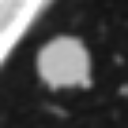
\includegraphics[width=\textwidth]{Fig/image_1.png}
    \caption{GT: Solid / Benign \quad Pred: Solid / Malignant}
  \end{subfigure}
  \hfill
  \begin{subfigure}[b]{0.45\textwidth}
    \centering
    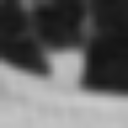
\includegraphics[width=\textwidth]{Fig/image_2.png}
    \caption{GT: Solid / Malignant \quad Pred: Solid / Malignant}
  \end{subfigure}

  \vspace{1em}

  \begin{subfigure}[b]{0.45\textwidth}
    \centering
    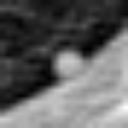
\includegraphics[width=\textwidth]{Fig/image_3.png}
    \caption{GT: Solid / Benign \quad Pred: Solid / Malignant}
  \end{subfigure}
  \hfill
  \begin{subfigure}[b]{0.45\textwidth}
    \centering
    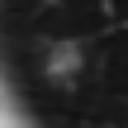
\includegraphics[width=\textwidth]{Fig/image_4.png}
    \caption{GT: Ground-Glass / Malignant \quad Pred: Solid / Benign}
  \end{subfigure}
  
  \caption{Qualitative results of the proposed model for nodule classification. Each example compares the ground truth (GT) and predicted (Pred) labels for nodule texture and malignancy.}
  \label{fig:qualitative}
\end{figure}


\section{Discussion}

\subsection{Hypothesis Evaluation}

The central hypothesis of this work was that soft parameter sharing via cross-talk between a texture branch and a malignancy branch would improve overall diagnostic performance compared to training each task in isolation. The experimental results do not support this hypothesis under the conditions evaluated.

For texture classification, all three models: STL, MTL cross-stitch, and MTL co-attention produce identical predictions, collapsing entirely to the solid majority class. The macro F1 of 0.33 reported across the board does not reflect a genuine representational equivalence between the models; it reflects the fact that 97 of 101 test samples are solid, making majority-class prediction nearly indistinguishable from high accuracy. The cross-talk mechanism cannot improve texture classification when the supervision signal itself is too imbalanced to provide a learning gradient for minority classes.

For malignancy prediction, the cross-stitch variant achieves a marginally higher malignant-class F1 than STL (0.74 vs.\ 0.72), but at the cost of substantially lower benign recall (0.24 vs.\ 0.32), resulting in a slightly lower macro F1 (0.55 vs.\ 0.56). The co-attention variant performs worse than STL on every metric. The hypothesis that biologically correlated tasks would benefit from shared representations is therefore not confirmed: rather than providing a useful inductive bias, the cross-task signal appears to act as noise that reinforces the model's existing bias toward the malignant majority class.

This outcome is consistent with the known risk of negative transfer in MTL, particularly when the auxiliary task (texture) provides a degenerate supervision signal. When the texture branch learns nothing beyond ``predict solid always'', the information it passes to the malignancy branch through the cross-talk units carries no useful gradient, and may actively interfere with the more informative malignancy signal.

\subsection{Conclusion}

This chapter proposed and evaluated \textit{MultiTaskCrossTalkNet}, a multi-task convolutional architecture that jointly predicts nodule texture category and malignancy risk from 2D CT crops via learnable cross-talk between task-specific branches. Two cross-talk mechanisms were compared against a single-task baseline: a cross-stitch unit performing global linear mixing of feature streams, and a co-attention unit performing channel-selective gating based on descriptors from the opposing branch.

Under the experimental conditions evaluated (508 samples drawn from the LIDC-IDRI dataset with severe solid-class dominance) neither MTL variant improved consistently over the STL baseline. The texture task proved unlearnable for minority classes regardless of architecture, and the malignancy task showed no reliable benefit from cross-task information sharing. The primary bottleneck was data quality and class distribution rather than architectural design.

These findings suggest that the value of cross-talk mechanisms in medical imaging MTL is contingent on the quality and balance of supervision available for each task. Future work should prioritize class-balanced sampling strategies, volumetric input representations, and the restoration of the progression task via a corrected data linkage, the condition under which the multi-task hypothesis is most likely to yield measurable gains.